\documentclass[aspectratio=169, 11pt]{beamer}

% --- Packages & Setup ---
\usepackage[utf8]{inputenc}
\usepackage[T1]{fontenc}
\usepackage{helvet}
\renewcommand{\familydefault}{\sfdefault}
\usepackage{xcolor}
\usepackage{booktabs}
\usepackage{graphicx}
\usepackage{tikz}
\usetikzlibrary{calc}

\graphicspath{{../}{./}}

% --- Branding Colors ---
\definecolor{amritaMaroon}{HTML}{A4123F}

% --- Theme Setup ---
\usetheme{Madrid}
\usecolortheme[named=amritaMaroon]{structure}
\setbeamertemplate{navigation symbols}{}
\setbeamertemplate{footline}[frame number]

% Reduce block padding globally to prevent vertical overflow
\addtobeamertemplate{block begin}{\vspace*{-2pt}}{\vspace*{-2pt}}
\addtobeamertemplate{block end}{}{\vspace*{-4pt}}

\begin{document}

% =========================================================================
% TITLE SLIDE (Research-Based Project)
% =========================================================================
\begin{frame}
    \begin{tikzpicture}[remember picture,overlay]
        \node[fill=amritaMaroon, text=white, font=\bfseries\footnotesize, anchor=north east, rounded corners=2pt, inner sep=5pt]
        at ($(current page.north east) + (-0.2cm,-0.2cm)$)
        {Type 1: Research Project};
    \end{tikzpicture}

    \centering
    \includegraphics[width=2.5cm]{logo.png}
    \vspace{0.05cm}

    {\large \textbf{\textcolor{amritaMaroon}{
    EvoSynth: Dynamic Multi-Armed Bandit Meta-Optimizer for\\
    Automated Model Selection and Hyperparameter Tuning
    }}} \\
    \vspace{0.05cm}
    {\footnotesize \textbf{23CSE498 -- Project Phase II (External Review)} \quad | \quad \textbf{Team Number: [2]}} \\
    \vspace{0.1cm}

    % Student Table
    \begin{table}
        \centering
        \footnotesize
        \renewcommand{\arraystretch}{1.05}
        \begin{tabular}{|c|c|l|}
            \hline
            \textbf{S.No} & \textbf{Register Number} & \textbf{Student Name} \\
            \hline
            1 & CB.SC.U4CSE23445 & Shivam Kharat \\
            \hline
            2 & CB.SC.U4CSE23565 & Siddharth Ladda \\
            \hline
            3 & CB.SC.U4CSE23627 & Kaushal Loya \\
            \hline
            4 & CB.SC.U4CSE23639 & Paarthu Reddy \\
            \hline
            5 & CB.SC.U4CSE23642 & Priyansh Narang \\
            \hline
        \end{tabular}
    \end{table}
    \vspace{0.05cm}

    {\footnotesize Guide: \textbf{Dr. Thangavelu S.}, Associate Professor, Department of CSE} \\
    {\scriptsize \today}
\end{frame}

% =========================================================================
% SLIDE 2: GUIDE APPROVAL EMAIL CONFIRMATION (Mandatory)
% =========================================================================
\begin{frame}{Guide Review \& Submission Approval}
    \framesubtitle{Confirmation of Project Review and Approval from Guide}
    \centering
    \begin{figure}
        \centering
        \includegraphics[
            width=0.80\textwidth,
            height=0.68\textheight,
            keepaspectratio
        ]{approval.png}
    \end{figure}
\end{frame}

% =========================================================================
% SECTION 1: PROBLEM DEFINITION, RESEARCH MOTIVATION & SOLUTION DESIGN
% =========================================================================
\section{Problem \& Solution Design}

% --- SLIDE 1: PROBLEM DEFINITION & RESEARCH MOTIVATION ---
\begin{frame}{1. Problem Definition \& Research Motivation}
    \framesubtitle{Problem Statement, Identified Literature Gap \& Objectives}

    \begin{block}{Problem Statement}
        \scriptsize
        \begin{itemize}
            \setlength{\itemsep}{1pt}
            \item \textbf{Core Problem:} AutoML systems rely on a single fixed optimizer that stagnates on non-convex hyperparameter landscapes---wasting search compute.
            \item \textbf{Domain Context:} By the No Free Lunch theorem, no single optimizer dominates everywhere; adaptive strategy switching is required.
        \end{itemize}
    \end{block}

    \begin{block}{Existing Limitations \& Research Gap}
        \scriptsize
        \begin{itemize}
            \setlength{\itemsep}{1pt}
            \item \textbf{Existing Methods:} Optuna (single Bayesian), FLAML (cost-frugal greedy), H2O (sequential Bayesian + heavy 10-model stacking).
            \item \textbf{Research Gap:} Lack of frameworks running concurrent optimizers with live stagnation detection and dynamic strategy swaps into a single model.
        \end{itemize}
    \end{block}

    \begin{block}{Research Objectives}
        \scriptsize
        \begin{itemize}
            \setlength{\itemsep}{1pt}
            \item \textbf{Objective 1:} UCB1 multi-armed bandit meta-engine routing budget to the best optimizer in real time.
            \item \textbf{Objective 2:} Live strategy switching (tier SWAPs) driven by stagnation and diversity monitoring.
            \item \textbf{Objective 3:} Ensemble-level accuracy ($93.47\%$) with a single deployable model (zero ensemble overhead, 2\,ms latency).
        \end{itemize}
    \end{block}
\end{frame}

% --- SLIDE 2: PROPOSED METHODOLOGY & OVERALL WORKFLOW ---
\begin{frame}{2. Proposed Methodology \& Overall Workflow}
    \framesubtitle{End-to-End Research Methodology / System Workflow Architecture}
    \centering
    \begin{figure}
        \centering
        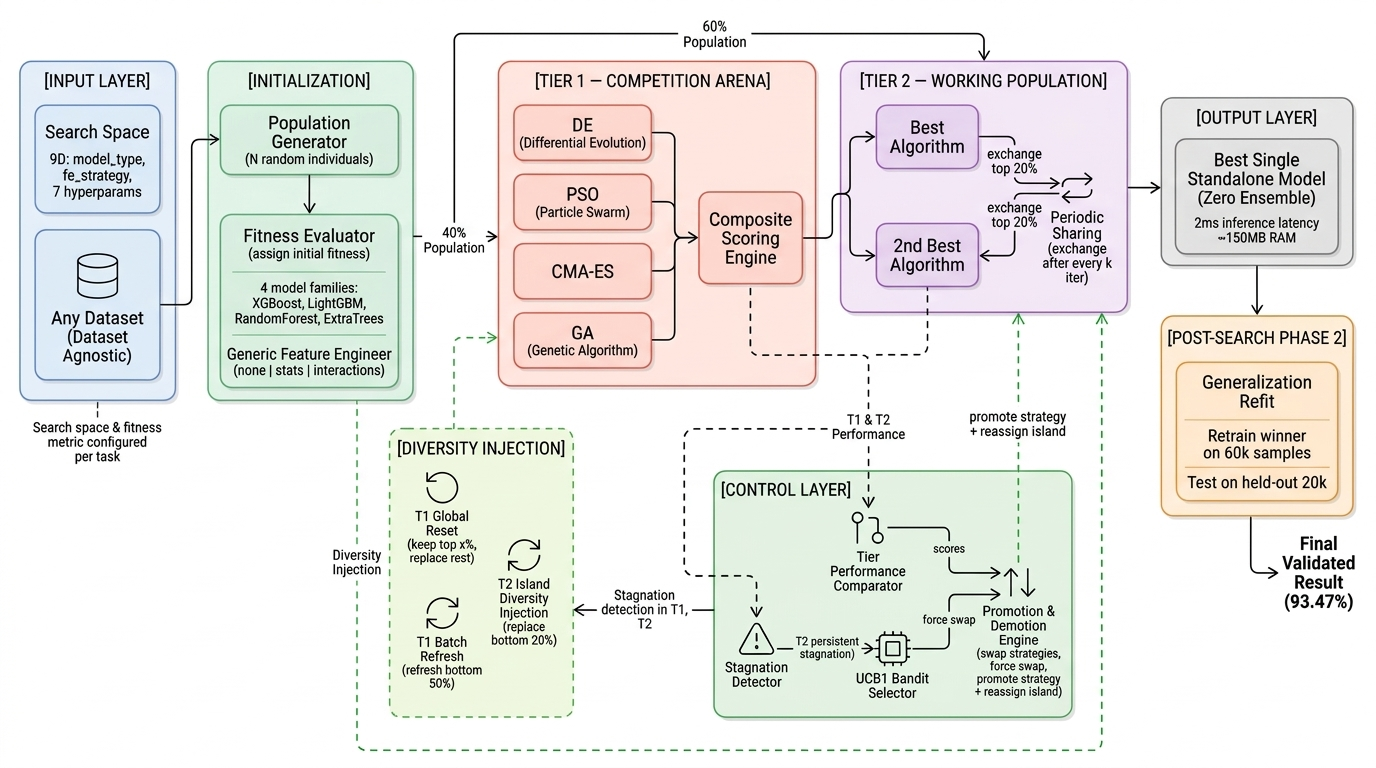
\includegraphics[
            width=0.82\textwidth,
            height=0.52\textheight,
            keepaspectratio
        ]{arch_updated.png}
    \end{figure}
    \vspace{-0.15cm}

    \begin{block}{Workflow Summary}
        \scriptsize
        Encode search space to $[0,1]^d$ $\to$ 40\% Tier-1 tournament (GA, PSO, DE, CMA-ES) $\to$ UCB1 selects top-2 $\to$ 60\% Tier-2 exploitation with elite sharing $\to$ Decode \& Evaluate (XGB/LGBM/RF/ExtraTrees + Generic FE) $\to$ Post-search refit on 60k $\to$ Single standalone model.
    \end{block}
\end{frame}

% --- SLIDE 3: METHODOLOGICAL COMPONENTS & FORMULATION ---
\begin{frame}{3. Methodological Components \& Formulation}
    \framesubtitle{Sub-Module Breakdown, Governing Mathematical Model \& Datasets}
    \begin{columns}[T]
        \column{0.49\textwidth}
        \begin{block}{Methodological Breakdown}
            \scriptsize
            \begin{itemize}
                \setlength{\itemsep}{1pt}
                \item \textbf{UCB1 Bandit Meta-Engine:} 5-metric composite rewards performance, diversity, and efficiency.
                \item \textbf{Two-Tier Island Model:} Tier-1 (40\%) competes 4 optimizers; top-2 promoted to Tier-2 (60\%) with elite sharing.
                \item \textbf{Stagnation Guard:} Zero-trend triggers random injection; live SWAP if a T1 algo leads T2 by $>10\%$.
            \end{itemize}
        \end{block}

        \begin{block}{Mathematical Formulation}
            \scriptsize
            \begin{itemize}
                \setlength{\itemsep}{1pt}
                \item \textbf{UCB1 Formula:} $UCB_i = CS_i + c\sqrt{\frac{\ln(E_{\text{total}})}{E_i}}$ \ ($c=0.1$)
                \item \textbf{Composite:} $CS = 0.30F + 0.25S + 0.15E + 0.15D + 0.15T$
                \item \textbf{Metrics:} $F$=Fit, $S$=Speed, $E$=Eff, $D$=Div, $T$=Trend
            \end{itemize}
        \end{block}

        \column{0.49\textwidth}
        \begin{block}{Dataset Specifications}
            \scriptsize
            \begin{itemize}
                \setlength{\itemsep}{1pt}
                \item \textbf{UCI Forest Covertype:} 581,012 samples, 54 features, 7 classes.
                \item \textbf{Protocol:} 20k search subsample (3-fold CV); 60k/20k train/test split for post-search generalization refit.
                \item \textbf{Feature Engineering:} Generic Feature Engineer with searchable strategies: \texttt{none}, \texttt{stats}, \texttt{interactions}.
            \end{itemize}
        \end{block}

        \begin{block}{Evaluation Metrics}
            \scriptsize
            \begin{itemize}
                \setlength{\itemsep}{1pt}
                \item \textbf{Accuracy:} Primary metric on held-out 20k test set.
                \item \textbf{Relative Error Reduction:} $(e_{\text{base}} - e_{\text{ours}}) / e_{\text{base}}$ ($64.6\%$).
                \item \textbf{Wall-Clock Time:} Total search + refit duration.
            \end{itemize}
        \end{block}
    \end{columns}
\end{frame}

% =========================================================================
% SECTION 2: IMPLEMENTATION COMPLETION (100%)
% =========================================================================
\section{Implementation Details}

% --- SLIDE 4: IMPLEMENTATION COMPLETION (100%) - OVERVIEW ---
\begin{frame}{4. Implementation Details -- Overview}
    \framesubtitle{Module-Wise Implementation \& Pipeline Integration Status}
    \vspace{-0.15cm}
    \begin{table}
        \centering
        \tiny
        \renewcommand{\arraystretch}{1.1}
        \begin{tabular}{p{3.2cm} p{7.4cm} c}
            \toprule
            \textbf{Module / Stage} & \textbf{Implemented Functionality} & \textbf{Status} \\
            \midrule
            Latent Space Mapping & Mixed params encoded to $[0,1]^d$; categoricals binned by $\lfloor zK\rfloor$ & 100\% (Integrated) \\
            Meta-Engine (UCB1) & Composite scoring, UCB1 bonus, promotion, swap + rollback & 100\% (Integrated) \\
            Worker Optimizers & Ask/Tell wrappers for GA, PSO, DE, CMA-ES & 100\% (Integrated) \\
            Tier Manager & 40/60 split, elite sharing, stagnation injection & 100\% (Integrated) \\
            Evaluators & XGBoost/LightGBM/RF/ExtraTrees + Generic FE + early stopping & 100\% (Functional) \\
            Generic Feature Engineer & Dataset-agnostic FE: \texttt{none}/\texttt{stats}/\texttt{interactions} & 100\% (Integrated) \\
            Live Telemetry Dashboard & FastAPI SSE stream into React (Vite + Tailwind) & 100\% (Integrated) \\
            \bottomrule
        \end{tabular}
    \end{table}
    \vspace{-0.2cm}

    \begin{block}{Implementation Environment \& Repository}
        \scriptsize
        \begin{itemize}
            \setlength{\itemsep}{1pt}
            \item \textbf{Compute Environment:} Python 3.14, XGBoost, LightGBM, scikit-learn, PyTorch, React (laptop CPU, zero GPU).
            \item \textbf{Repository \& Deliverables:} \href{https://github.com/paarthureddy/EvoSynth}{\textcolor{blue}{GitHub (branch PostReview2)}} \quad | \quad \href{https://evosynth-2027.github.io/evosynth-docs/}{\textcolor{blue}{Docs}} \quad | \quad \href{https://doi.org/10.5281/zenodo.23645119}{\textcolor{blue}{Zenodo Dataset}}
        \end{itemize}
    \end{block}
\end{frame}

% --- SLIDE 5: CORE MODULE IMPLEMENTATION DETAILS ---
\begin{frame}{5. Core Module Implementation Details}
    \framesubtitle{Two-Tier Control Logic, Parameter Configurations \& Interfaces}
    \begin{columns}[T]
        \column{0.52\textwidth}
        \begin{block}{Two-Tier Control Flow}
            \scriptsize
            \begin{itemize}
                \setlength{\itemsep}{1pt}
                \item \textbf{Init:} Population evaluated; 40\% Tier-1 / 60\% Tier-2 reserve.
                \item \textbf{Tier-1 Tournament:} GA, PSO, DE, CMA-ES compete across 10 iters.
                \item \textbf{Promotion:} Composite + UCB1 bonus ranks; top-2 move to Tier-2.
                \item \textbf{Live SWAP:} T1 algo replaces worst T2 one if it leads by $>10\%$.
                \item \textbf{Rollback:} Must beat global best within 5 iters, else reverted.
                \item \textbf{Elite Sharing:} Top 20\% of each T2 island pooled and shared.
            \end{itemize}
        \end{block}

        \begin{block}{Generic Feature Engineer}
            \scriptsize
            \begin{itemize}
                \setlength{\itemsep}{1pt}
                \item \textbf{Searchable Gene:} \texttt{fe\_strategy} $\in$ \{\texttt{none}, \texttt{stats}, \texttt{interactions}\}.
                \item \textbf{Dataset-Agnostic:} No domain-specific column names; pure tabular math.
            \end{itemize}
        \end{block}

        \column{0.46\textwidth}
        \centering
        {\scriptsize \textbf{\textcolor{amritaMaroon}{Default Parameter Setup}}}
        \vspace{0.05cm}
        \begin{table}
            \centering
            \tiny
            \renewcommand{\arraystretch}{1.0}
            \begin{tabular}{lc}
                \toprule
                \textbf{Parameter} & \textbf{Value} \\
                \midrule
                Evaluation budget & 120 (Covertype) \\
                Population size & 30 \\
                Tier-1 / Tier-2 split & 40\% / 60\% \\
                Tier-1 iterations & 10 \\
                Checkpoint interval $k$ & 5 \\
                Exploration constant $c$ & 0.1 \\
                Swap threshold & 10\% \\
                Rollback grace period & 5 iters \\
                Elite share & top 20\% \\
                Injection (T1 / T2) & 50\% / 20\% \\
                Search space dims & 9 (incl.\ model, FE) \\
                Model families & 4 (XGB, LGBM, RF, ET) \\
                \bottomrule
            \end{tabular}
        \end{table}
    \end{columns}
\end{frame}

% =========================================================================
% SECTION 3: PRELIMINARY VERIFICATION & DEMONSTRATION
% =========================================================================
\section{Verification \& Demonstration}

% --- SLIDE 6: PRELIMINARY VERIFICATION & QUANTITATIVE RESULTS ---
\begin{frame}{6. Preliminary Verification \& Quantitative Results}
    \framesubtitle{UCI Forest Covertype Benchmark (581,012 samples, 54 features, 7 classes)}
    \begin{table}
        \centering
        \scriptsize
        \renewcommand{\arraystretch}{1.15}
        \begin{tabular}{p{4.8cm} c c c}
            \toprule
            \textbf{Method / Configuration} & \textbf{Model} & \textbf{Time} & \textbf{Accuracy} \\
            \midrule
            Default Baseline (XGBoost) & Untuned XGBoost & 2\,s & 80.97\% \\
            Default Baseline (LightGBM) & Untuned LightGBM & 1\,s & 81.07\% \\
            Default Baseline (RandomForest) & Untuned RF & 3\,s & 81.48\% \\
            \midrule
            EvoSynth Search (20k, 3-fold CV) & ExtraTrees + FE & 8m 30s & 86.39\% \\
            \textbf{EvoSynth Final (60k/20k refit)} & \textbf{ExtraTrees} & \textbf{9m 44s} & \textbf{93.47\%} \\
            \bottomrule
        \end{tabular}
    \end{table}
    \vspace{-0.15cm}

    \begin{block}{Experimental Verification Summary}
        \scriptsize
        \begin{itemize}
            \setlength{\itemsep}{1.5pt}
            \item \textbf{Quantitative Findings:} 93.47\% accuracy = \textbf{64.6\% relative error reduction} (19\% $\to$ 6.53\% error) over untuned baselines, using a single deployable model.
            \item \textbf{Verification of Core Hypothesis:} Dynamic SWAP confirmed---Iteration 2: $T1\_PSO$ (UCB 0.720, diversity 0.500) replaced $T2\_GA$ (UCB 0.547, diversity 0.450), proving live strategy switching improves convergence under stagnation.
        \end{itemize}
    \end{block}
\end{frame}

% --- SLIDE 7: EXPERIMENTAL VISUALIZATIONS & PROTOTYPE DEMONSTRATION ---
\begin{frame}{7. Comparison with Existing Frameworks \& Demonstration}
    \framesubtitle{Positioning EvoSynth against Optuna, FLAML, and H2O AutoML}

    \vspace{-0.25cm}
    \begin{table}
        \centering
        \tiny
        \setlength{\tabcolsep}{3.5pt}
        \renewcommand{\arraystretch}{1.1}
        \resizebox{\textwidth}{!}{%
        \begin{tabular}{p{2.3cm} p{2.6cm} p{2.5cm} p{2.7cm} p{3.2cm}}
            \toprule
            \textbf{Aspect} & \textbf{Optuna} & \textbf{FLAML} & \textbf{H2O AutoML} & \textbf{EvoSynth (Ours)} \\
            \midrule
            Search paradigm & Single Bayesian (TPE/CMA) & Cost-frugal local search & Random/Bayesian search & \textbf{UCB1 Multi-Armed Bandit} \\
            Search strategies & Fixed 1 sampler/study & Single greedy method & Sequential single trial & \textbf{4 concurrent (GA,PSO,DE,CMA)} \\
            Strategy switching & None (static sampler) & None & None & \textbf{Dynamic Tier SWAPs ($>10\%$)} \\
            Diversity protection & None & None & None & \textbf{Pop.\ Diversity in UCB1} \\
            Feature engineering & Manual & Limited heuristics & Fixed preprocessing & \textbf{Dataset-Agnostic Gene} \\
            Production output & Single model & Single model & Heavy 10-model stack & \textbf{Single model (2\,ms, 150MB)} \\
            \bottomrule
        \end{tabular}%
        }
    \end{table}
    \vspace{-0.2cm}

    \begin{block}{Demonstration Overview}
        \scriptsize
        \begin{itemize}
            \setlength{\itemsep}{1pt}
            \item \textbf{Pareto Advantage:} Delivers ensemble-level accuracy (93.47\%) without latency/RAM costs of heavy stacking ensembles.
            \item \textbf{Live Demo:} \texttt{run\_covertype.py} runs end-to-end with real-time React dashboard displaying UCB1 metrics \& SWAPs.
            \item \textbf{Vision NAS:} PyTorch CNN on Handwritten Digits reached \textbf{95.78\%} in 80 evals (17.7\,s), verifying cross-domain versatility.
        \end{itemize}
    \end{block}
\end{frame}

% =========================================================================
% SECTION 4: TECHNICAL KNOWLEDGE & VIVA VOCE
% =========================================================================
\section{Technical Knowledge}

% --- SLIDE 8: TECHNICAL JUSTIFICATION, DESIGN TRADE-OFFS & INSIGHTS ---
\begin{frame}{8. Technical Justification, Design Trade-offs \& Insights}
    \framesubtitle{Methodological Rationale, Trade-offs \& Boundary Conditions}
    \begin{columns}[T]
        \column{0.49\textwidth}
        \begin{block}{1. Methodological Justification}
            \scriptsize
            \begin{itemize}
                \setlength{\itemsep}{1pt}
                \item No single optimizer wins everywhere (NFL). UCB1 routes trials to the leader while exploration bonus prevents early trap.
                \item Two-tier structure separates exploration (T1) from exploitation (T2), balancing the explore-exploit tradeoff.
            \end{itemize}
        \end{block}

        \begin{block}{2. Design \& Parameter Trade-offs}
            \scriptsize
            \begin{itemize}
                \setlength{\itemsep}{1pt}
                \item \textit{Latent Space:} Slight decode overhead, but enables continuous optimizers (PSO/CMA-ES) to tune categoricals.
                \item \textit{Meta-overhead:} $<0.05\%$ of total time; 99.95\% spent on model training.
                \item \textit{Offline Meta-Optimization:} Zero inference latency penalty.
            \end{itemize}
        \end{block}

        \column{0.49\textwidth}
        \begin{block}{3. Boundary Conditions \& Edge Cases}
            \scriptsize
            \begin{itemize}
                \setlength{\itemsep}{1pt}
                \item Rollback guard: Swapped-in algo must beat global best in 5 iters, else reverted.
                \item Stagnation rescue: Zero-trend triggers random injection in both tiers.
                \item Robust under 30\% label-noise benchmark ($\approx$79.4\% best).
            \end{itemize}
        \end{block}

        \begin{block}{4. Limitations \& Future Scope}
            \scriptsize
            \begin{itemize}
                \setlength{\itemsep}{1pt}
                \item \textit{Current:} Single-machine execution; FE focused on tabular data.
                \item \textit{Future Scope:} Distributed workers via Ray; warm-start meta-learning across datasets; deep learning pipeline NAS.
            \end{itemize}
        \end{block}
    \end{columns}
\end{frame}

% =========================================================================
% TECHNICAL ENRICHMENT
% =========================================================================
\section{Technical Enrichment}
\begin{frame}{Technical Enrichment Activity}
    \framesubtitle{Professional Online Certification Details (Individual Mandatory: 10--20 Hours)}
    \vspace{-0.1cm}
    \begin{table}
        \centering
        \footnotesize
        \renewcommand{\arraystretch}{1.15}
        \begin{tabular}{|c|p{2.8cm}|p{5.0cm}|p{2.0cm}|c|}
            \hline
            \textbf{S.No} & \textbf{Student Name} & \textbf{Chosen MOOC / Course Title} & \textbf{Platform} & \textbf{Hours} \\
            \hline
            1 & Shivam Kharat & Evolutionary Computation and its Applications & Coursera & 10 Hrs \\
            \hline
            2 & Siddharth Ladda & Evolutionary Computation and its Applications & Coursera & 10 Hrs \\
            \hline
            3 & Kaushal Loya & Evolutionary Computation and its Applications & Coursera & 10 Hrs \\
            \hline
            4 & Paarthu Reddy & Front-End Web Development with React (Dashboard) & Coursera & 10 Hrs \\
            \hline
            5 & Priyansh Narang & Optimization for ML (Mathematical Latent Space) & NPTEL & 10 Hrs \\
            \hline
        \end{tabular}
    \end{table}
\end{frame}

% =========================================================================
% REFERENCES & THANK YOU
% =========================================================================
\setbeamertemplate{bibliography item}{\insertbiblabel}

\section{References}

\begin{frame}[allowframebreaks]{References}
\fontsize{6.5}{8}\selectfont
\begin{thebibliography}{99}

\bibitem{ref1}
A. Scrivano, ``The Emergence of Automated Machine Learning (AutoML): Trends and Future Prospects,'' \textit{Research Square}, 2025.

\bibitem{ref2}
E. Alcoba\c{c}a and A. C. P. L. F. de Carvalho, ``A Literature Review on Automated Machine Learning,'' \textit{Artificial Intelligence Review}, Springer, 2025.

\bibitem{ref3}
E. L. Estevanell-Valladares \textit{et al.}, ``XAutoLM: Efficient Fine-Tuning of Language Models via Meta-Learning and AutoML,'' in \textit{Proc. Empirical Methods in Natural Language Processing (EMNLP)}, 2025, pp. 7863--7880.

\bibitem{ref4}
G. Borboudakis, P. Charonyktakis, K. Paraschakis, and I. Tsamardinos, ``A Meta-Level Learning Algorithm for Sequential Hyper-Parameter Space Reduction in AutoML,'' \textit{arXiv preprint arXiv:2312.06305}, 2024.

\bibitem{ref5}
M. Crepin\v{s}ek \textit{et al.}, ``Overcoming Stagnation in Metaheuristic Algorithms with MsMA's Adaptive Meta-Level Partitioning,'' \textit{Mathematics}, vol. 13, no. 11, p. 1803, 2025.

\bibitem{ref6}
M. Gerber, A. S. Bosman, and J. P. de Villiers, ``Online Meta-Learning for AutoML in Real-Time,'' \textit{arXiv preprint arXiv:2502.20279}, 2025.

\bibitem{ref7}
P. Auer, N. Cesa-Bianchi, and P. Fischer, ``Finite-time analysis of the multiarmed bandit problem,'' \textit{Machine Learning}, vol. 47, no. 2, pp. 235--256, 2002.

\bibitem{ref8}
D. H. Wolpert and W. G. Macready, ``No free lunch theorems for optimization,'' \textit{IEEE Trans. Evolutionary Computation}, vol. 1, no. 1, pp. 67--82, 1997.

\bibitem{ref9}
C. Wang, Q. Wu, M. Weimer, and E. Zhu, ``FLAML: A fast and lightweight AutoML library,'' \textit{Proc. Machine Learning and Systems}, vol. 3, pp. 434--447, 2021.

\bibitem{ref10}
E. LeDell and S. Poirier, ``H2O AutoML: Scalable automatic machine learning,'' in \textit{ICML Workshop on Automated Machine Learning}, 2020.

\end{thebibliography}
\end{frame}

\begin{frame}
    \centering
    {\Huge \textbf{\textcolor{amritaMaroon}{Thank You}}} \\[0.4cm]
    {\large \textbf{Questions \& Viva Voce}}
\end{frame}

\end{document}
